\begin{figure}

        \centering

        \begin{subfigure}[b]{0.45\textwidth}
                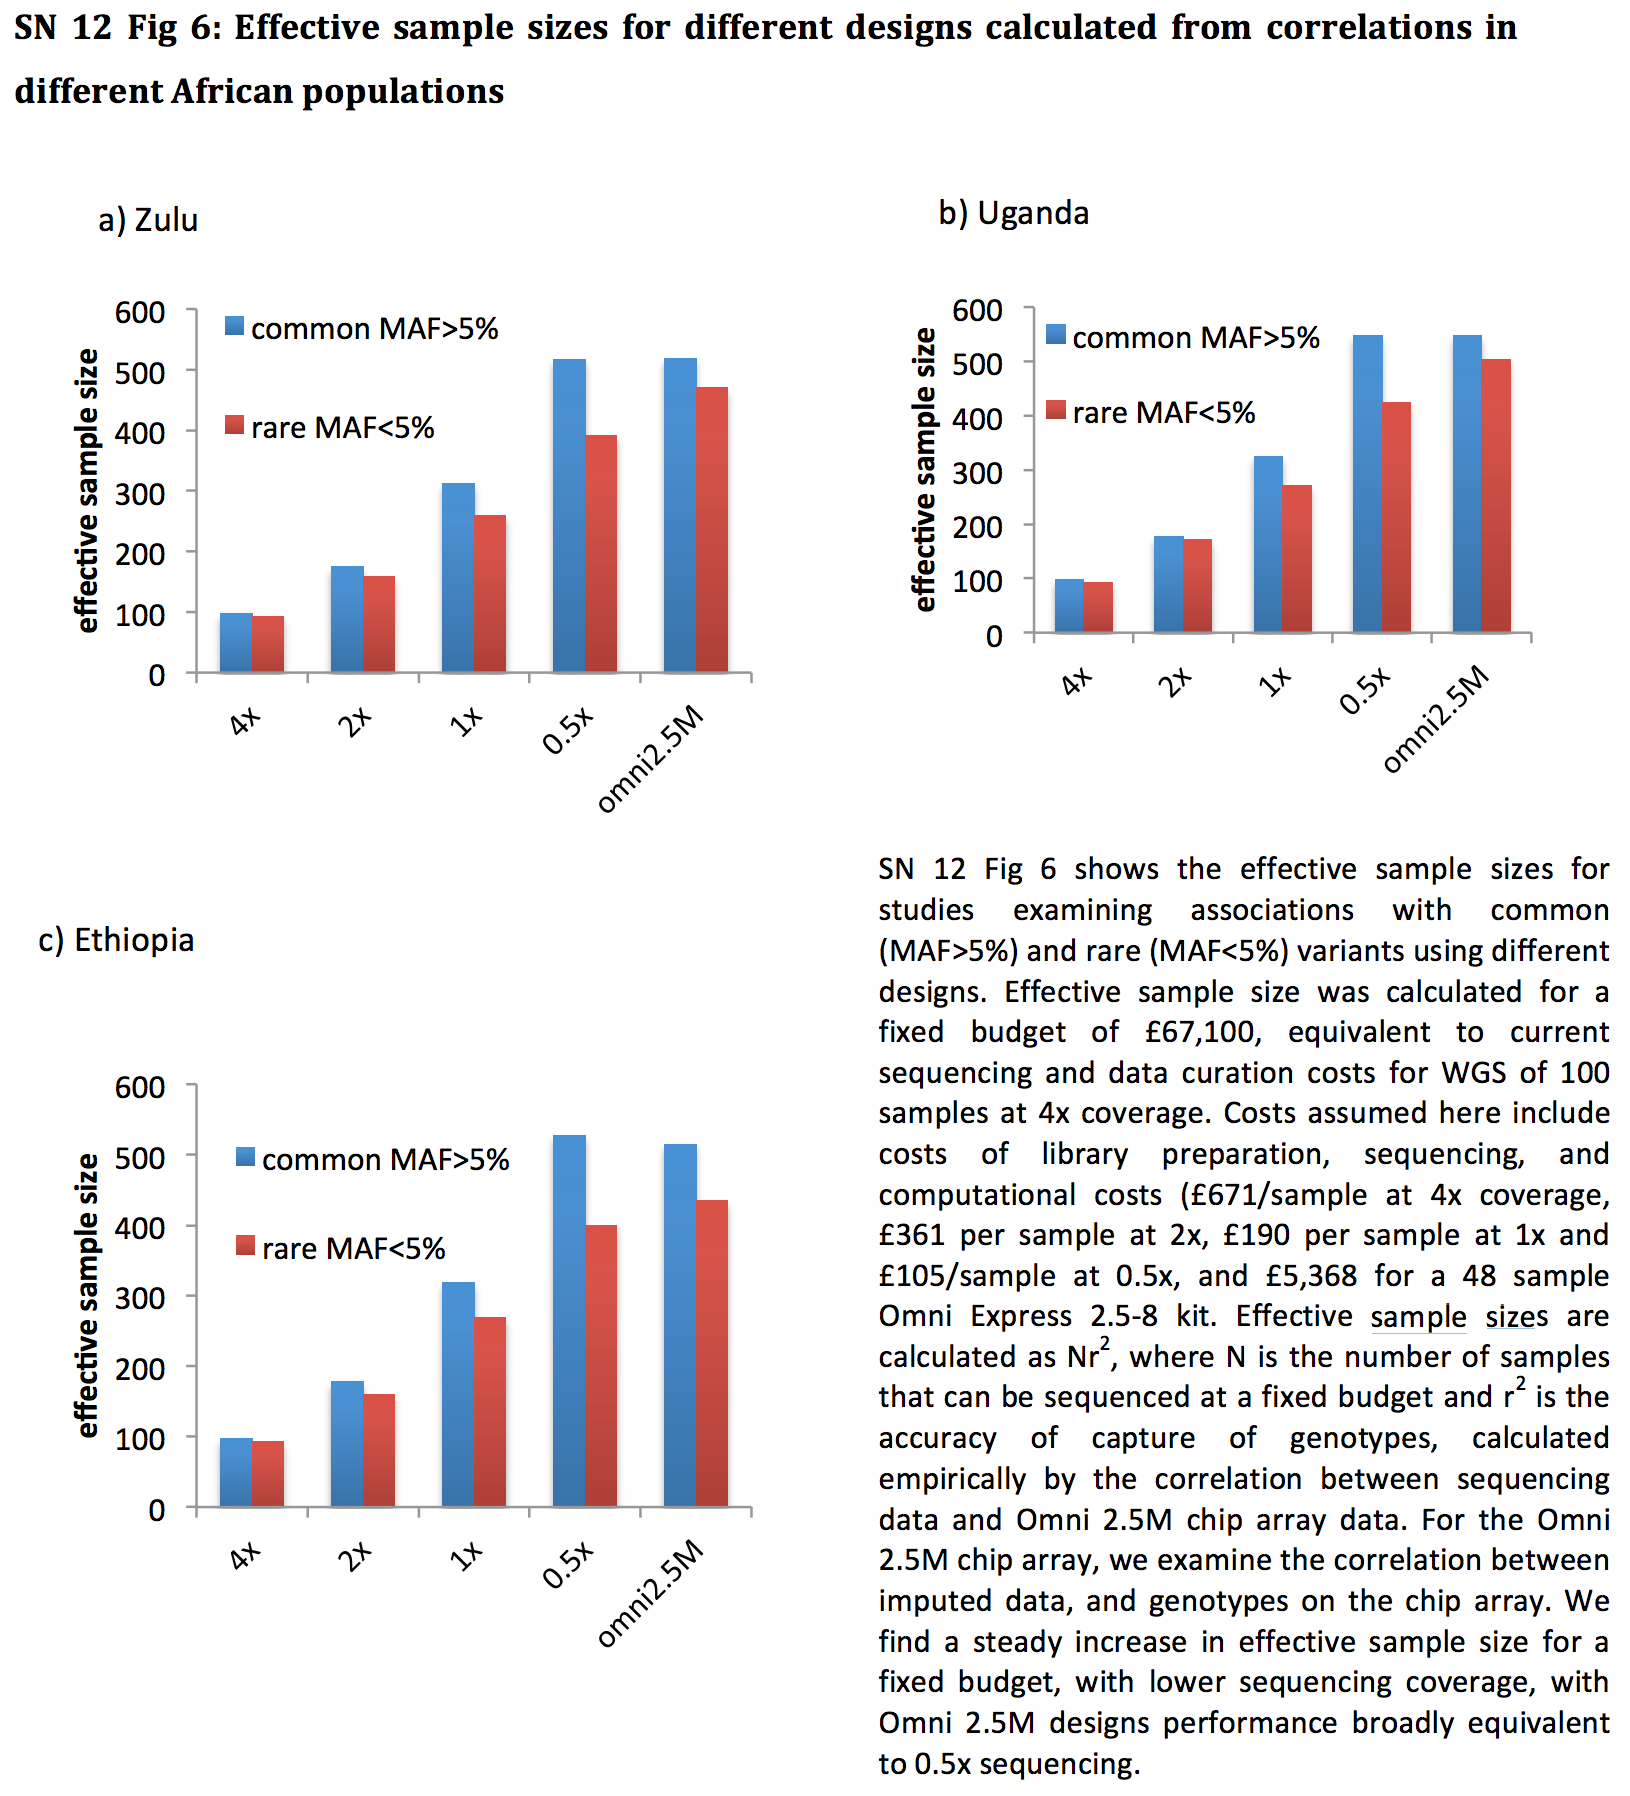
\includegraphics[trim={14.5cm 17.5cm 1.5cm 4.75cm},clip,width=0.95\textwidth]{fig/SN12f6}
                \caption{Uganda}
                \label{fig:SN12f6uganda}
        \end{subfigure}%

        \begin{subfigure}[b]{0.45\textwidth}
                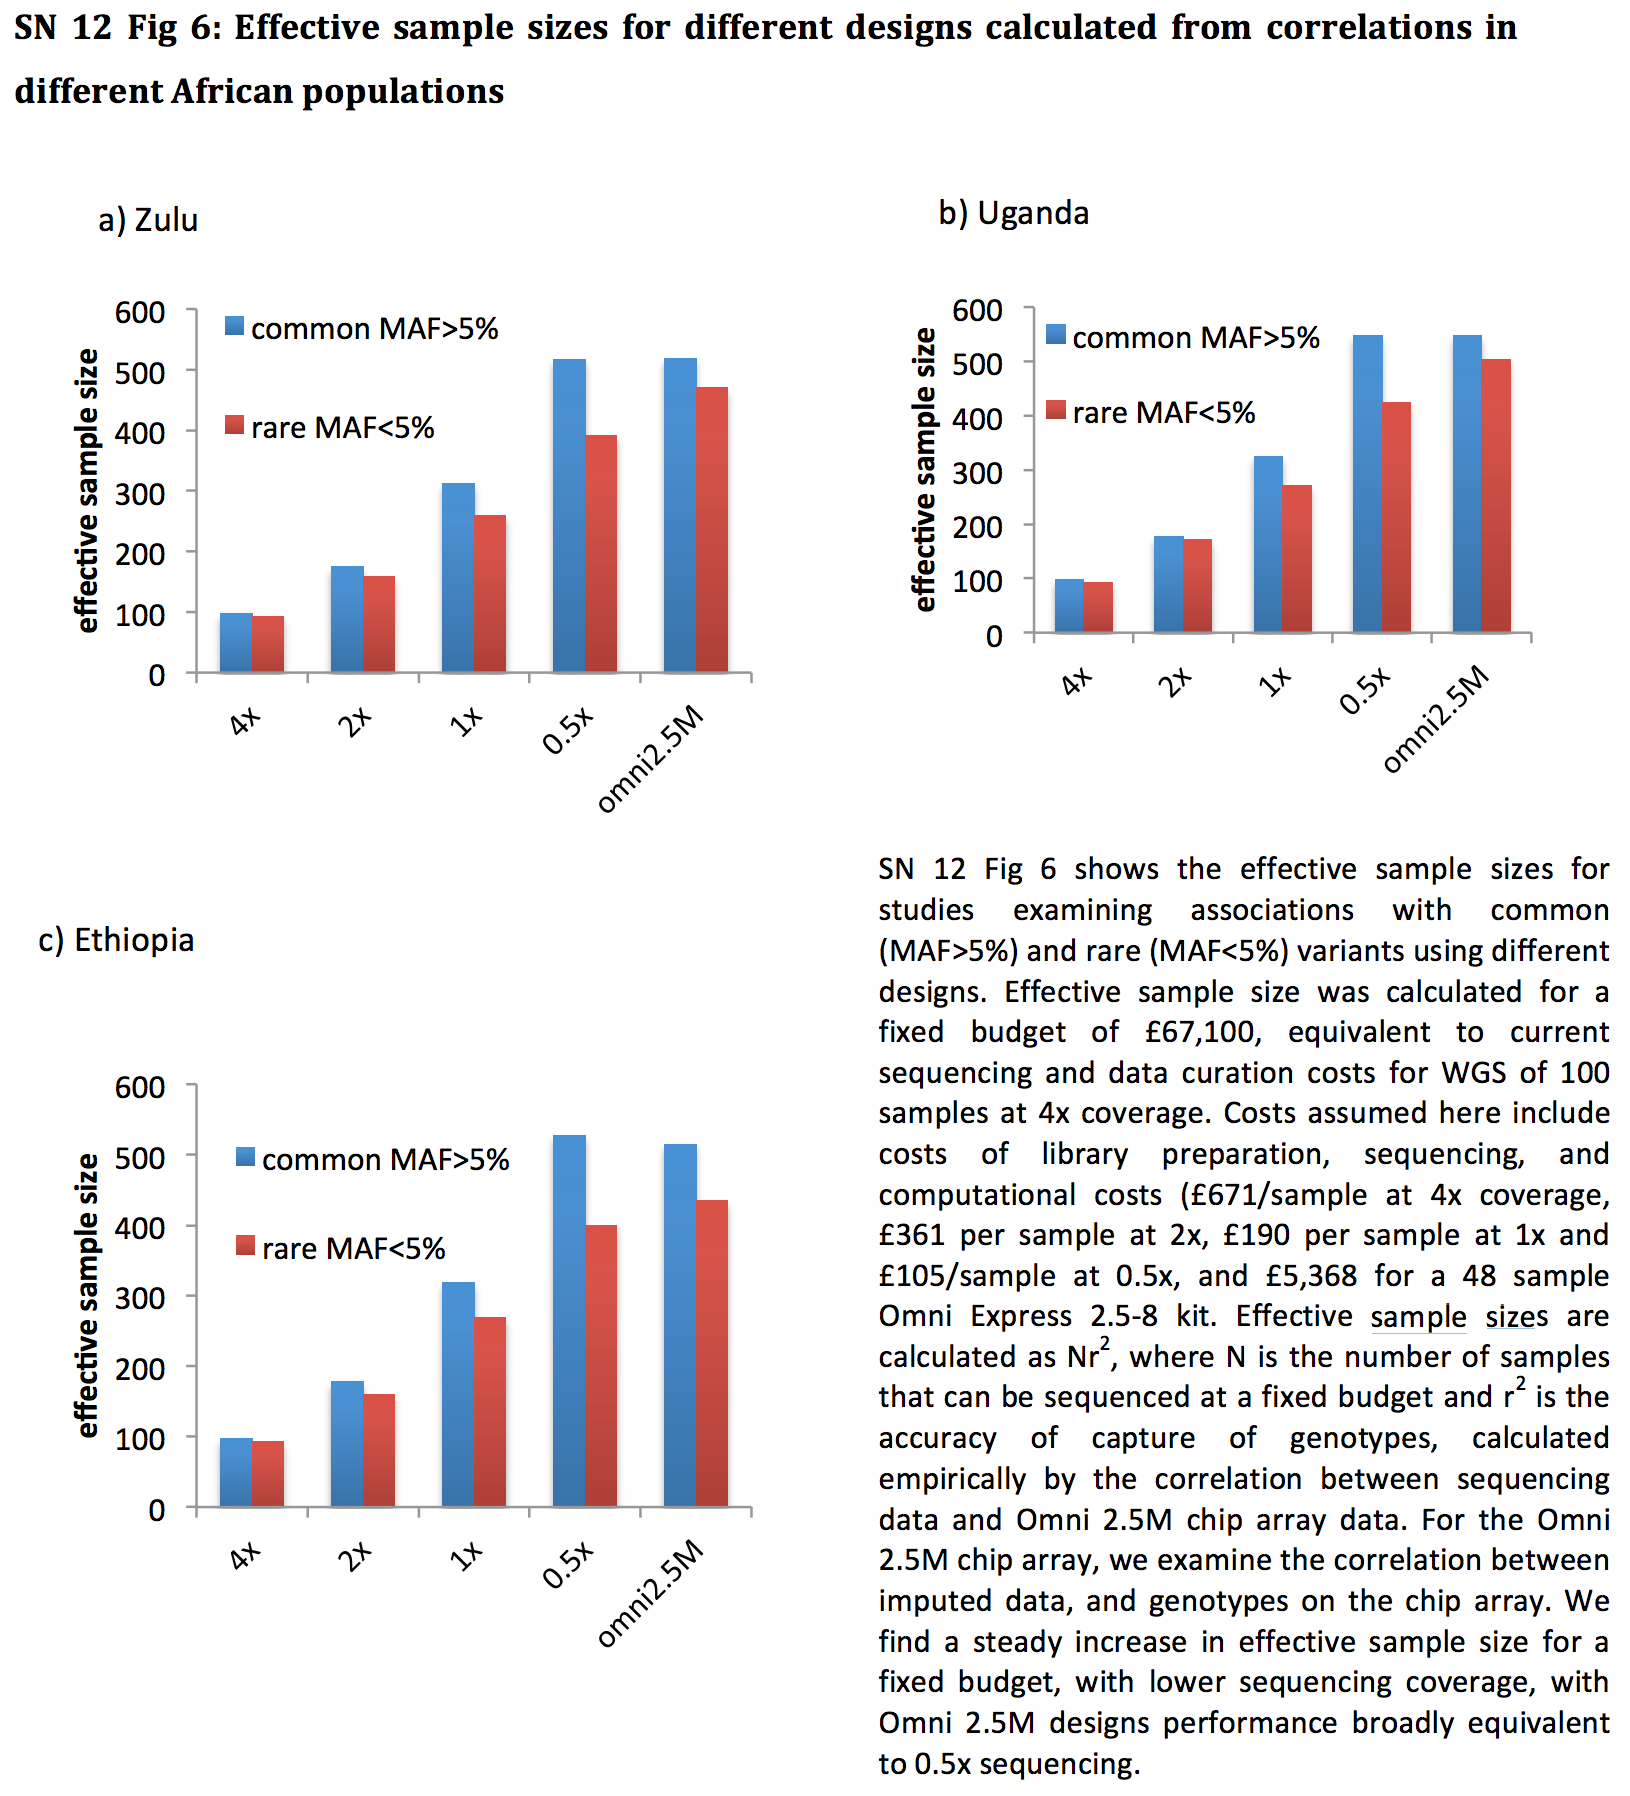
\includegraphics[trim={0 17cm 16cm 4.75cm},clip,width=0.9\textwidth]{fig/SN12f6}
                \caption{Zulu}
                \label{fig:SN12f6zulu}
        \end{subfigure}

        \begin{subfigure}[b]{0.45\textwidth}
                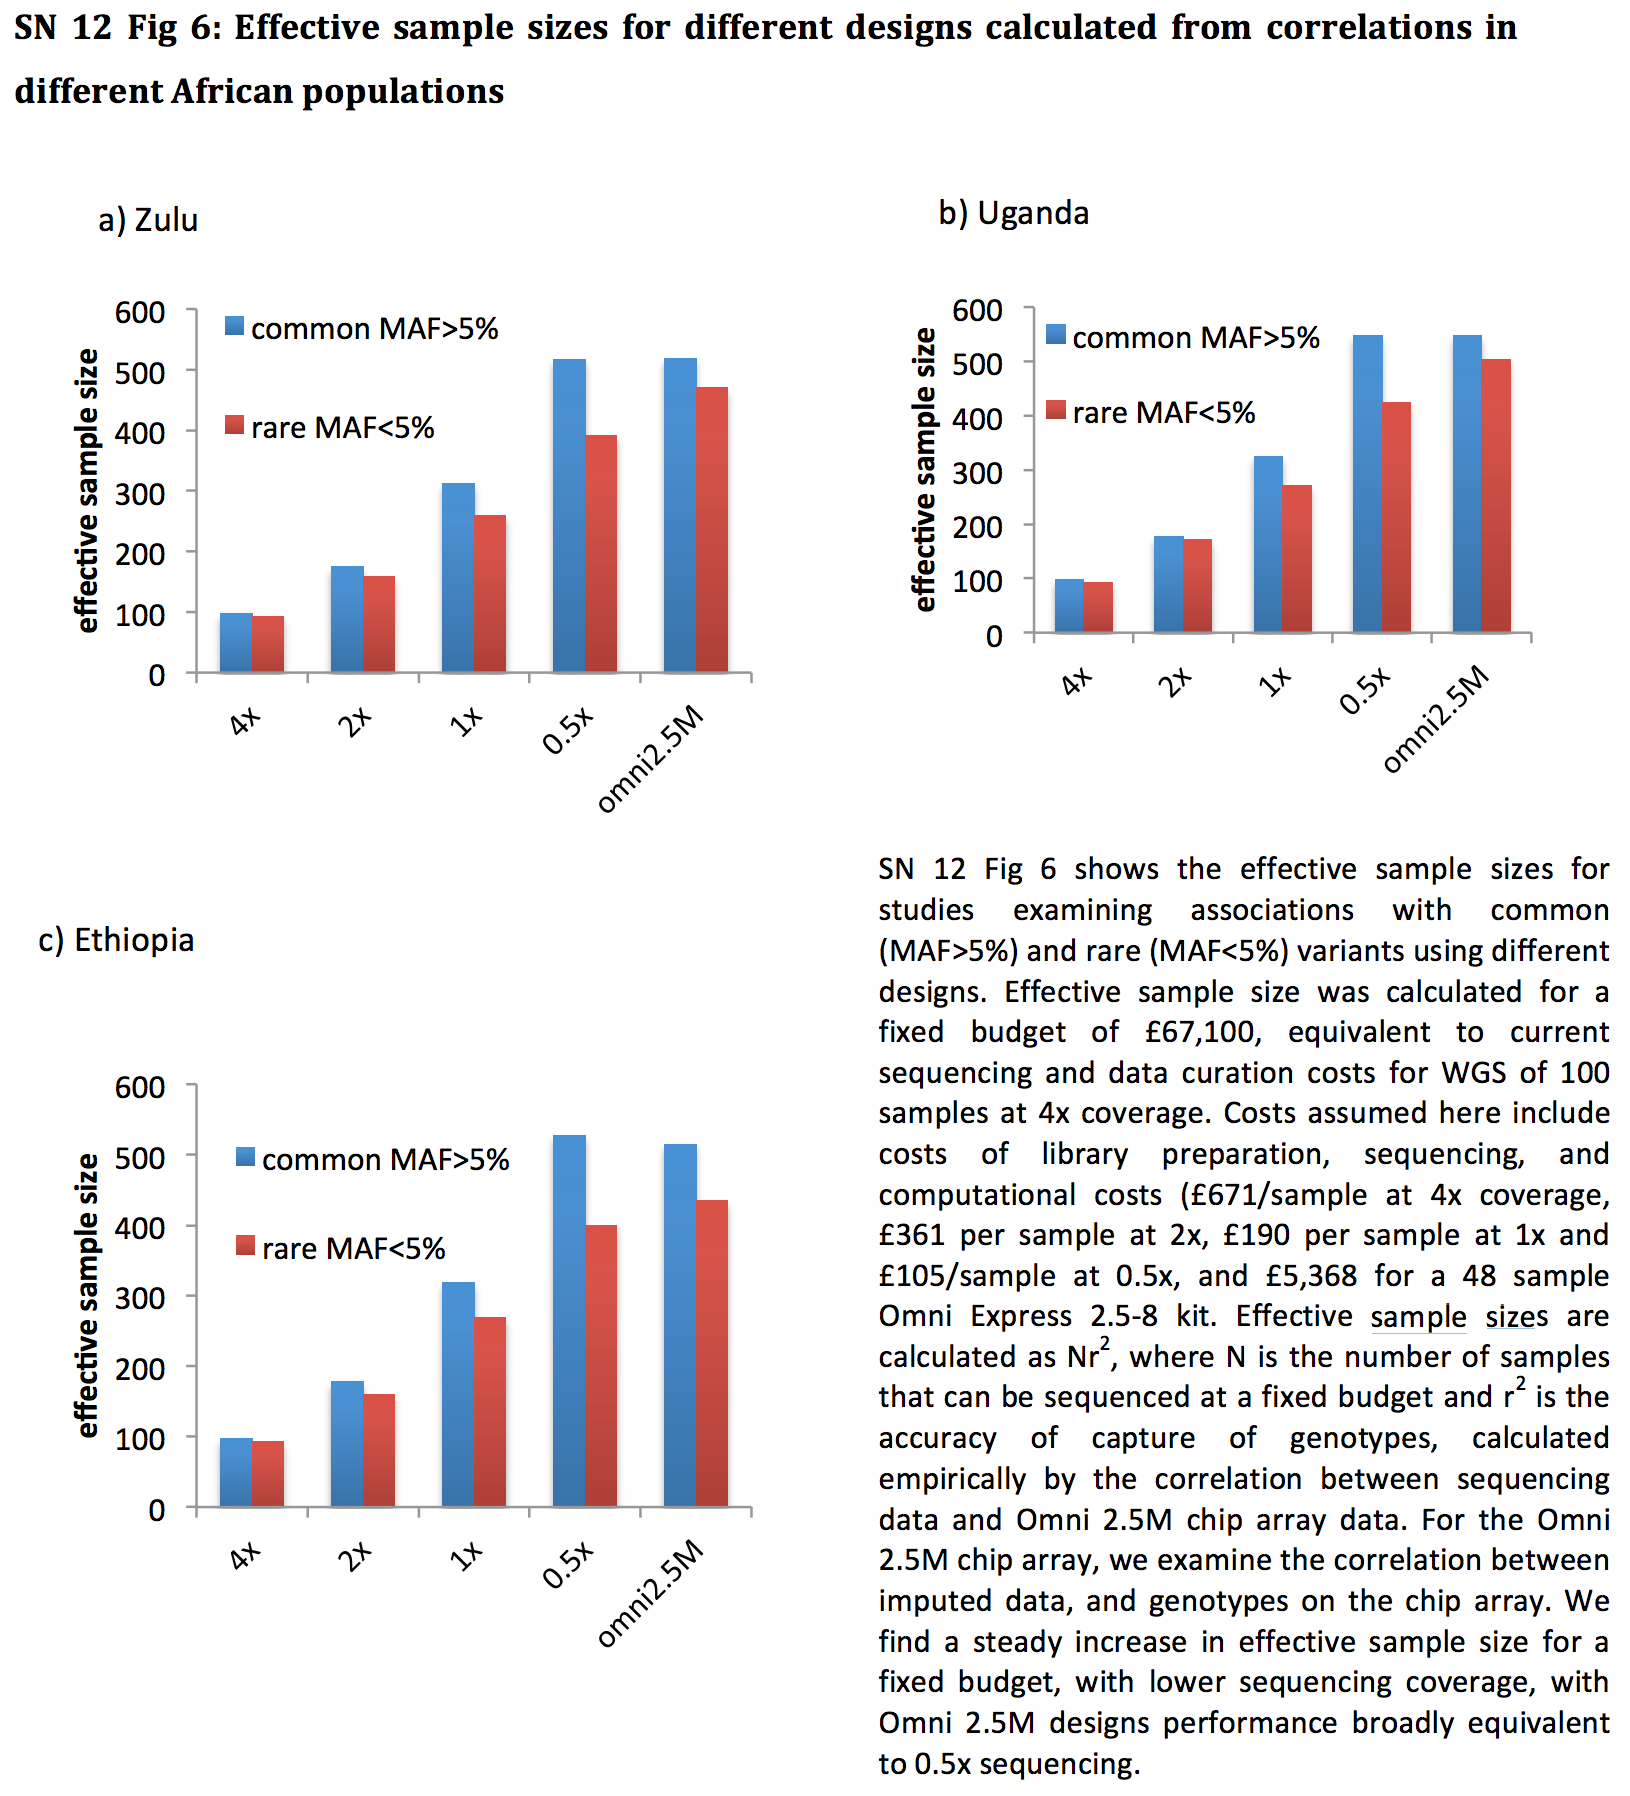
\includegraphics[trim={0 2cm 16cm 18cm},clip,width=0.9\textwidth]{fig/SN12f6}
                \caption{Ethiopia}
                \label{fig:SN12f6ethiopia}
        \end{subfigure}

        \caption[Effective samples sizes for down-sampled and imputed chip data.]{
        Effective sample sizes for studies examining associations with common (MAF>5\%) and rare (MAF<5\%) variants using different designs. Effective sample size was calculated for a fixed budget of £67,100, equivalent to current sequencing and data curation costs for \gls{WGS} of 100 samples at 4x coverage. Costs assumed here include costs of library preparation, sequencing, and computational costs (£671/sample at 4x coverage, £361 per sample at 2x, £190 per sample at 1x and £105/sample at 0.5x, and £5,368 for a 48 sample Omni 2.5-8 kit. Effective sample sizes are calculated as \textit{N}\textit{r}\textsuperscript{2}, where \textit{N} is the number of samples that can be sequenced at a fixed budget and \textit{r}\textsuperscript{2} is the accuracy of capture of genotypes, calculated empirically by the correlation between sequencing data and Omni 2.5M chip array data. For the Omni 2.5M chip array,we examine the correlation between imputed data, and genotypes on the chip array. We find a steady increase in effective sample size for a fixed budget, with lower sequencing coverage, with Omni 2.5M designs performance broadly equivalent to 0.5x sequencing.
        }

        \label{fig:SN12f6}

\end{figure}